\begin{figure}[h]
	\centering  
    \begin{tikzpicture}
    \node[inner sep=0pt] (pic) at (0,0)
    {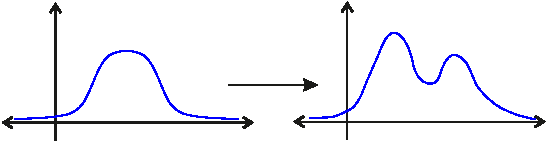
\includegraphics[width=12cm]{pictures/picture_2_3.pdf}};
    \draw [color=black](-0.8,0.5) node[anchor=north west] {$ \textbf{x} $ data};
    \draw [color={rgb,255:red,00; green,00; blue,255}](-3.5,1.2) node[anchor=north west] {$ \pi(\t) $};
    \draw [color={rgb,255:red,00; green,00; blue,255}](4.4,0.6) node[anchor=north west] {$ \pi(\t|\textbf{x}) $};
    \end{tikzpicture}
	\caption{Naznačení přechodu apriorní hustoty k aposteriorní hustotě pravděpodobnosti při daných datech.}
\end{figure}